\documentclass[a4paper,12pt]{article}
\usepackage{cmap}
\usepackage[T2A]{fontenc}
\usepackage[utf8]{inputenc}
\usepackage[english,russian]{babel}
\usepackage{listings}
\usepackage{amsmath}
\usepackage{amsfonts}
\usepackage{float}
\usepackage{csquotes}
\usepackage{graphicx}
\usepackage{hyphenat}
\usepackage{xcolor}
\usepackage{hyperref}
\usepackage{mathtools}
\usepackage{upgreek}


\renewcommand{\theequation}{\thesection.\arabic{equation}}


\author{Шерепа Никита}
\title{ThinkDSP. Лабораторная 6. Дискретное косинусное преобразование.}
\date{\today}

\graphicspath{{res/screenshots}}

\begin{document}%
	
	\maketitle
	
	\newpage \tableofcontents
	\newpage \listoffigures
	\newpage \lstlistoflistings
	
	\newpage
	
	\definecolor{dkgreen}{rgb}{0,0.6,0}
	\definecolor{gray}{rgb}{0.5,0.5,0.5}
	\definecolor{mauve}{rgb}{0.58,0,0.82}
	
	\lstset{
		language=Python,                 % выбор ЯП для подсветки 
		basicstyle=\small\sffamily, % размер и начертание шрифта для подсветки кода
		numbers=left,               % где поставить нумерацию строк (слева\справа)
		numberstyle=\tiny,           % размер шрифта для номеров строк
		stepnumber=1,                   % размер шага между двумя номерами строк
		numbersep=5pt,                % как далеко отстоят номера строк от подсвечиваемого кода
		aboveskip=3mm,
		belowskip=3mm,
		showstringspaces=false,
		columns=flexible,
		captionpos=b, 
		basicstyle={\small\ttfamily},
		numbers=left,
		numberstyle=\tiny\color{gray},
		keywordstyle=\color{blue},
		commentstyle=\color{mauve},
		stringstyle=\color{dkgreen},
		breaklines=true,
		breakatwhitespace=true,
		tabsize=3
	}


	\section {Упражение 6.1}
	
	\begin{enumerate} 
			
		\item \textbf{Задание}
		
		Убедитесь, что \texttt{analyze1} требует времени пропорционально \texttt{\(n^3\)}, а \texttt{analyze2} - пропорционально \texttt{\(n^2\)}. Для этого запустите их с несколькими разными массивами и засекайте время работы.
		
		\item \textbf{Ход работы}
		
		Для начала создадим сигнал и вычислим его \texttt{Shape}
		\begin{lstlisting}[caption=Создание сигнала и его \texttt{Shape}]
			from thinkdsp import UncorrelatedGaussianNoise
			
			signal = UncorrelatedGaussianNoise()
			noise = signal.make_wave(duration=1.0, framerate=16384)
			noise.ys.shape
			
			Output
			(16384,)
		\end{lstlisting}
		
		Следующая функция - \texttt{plot\_bests()} - отображает массив значений выстраивает из них прямую линию
		\begin{lstlisting}[caption=Функция \texttt{plot\_bests()}]
			def plot_bests(ns, bests):    
				plt.plot(ns, bests)
				decorate(**loglog)
				
				x = np.log(ns)
				y = np.log(bests)
				t = linregress(x,y)
				slope = t[0]
				
				return slope
		\end{lstlisting}
		
		Теперь поработаем с \texttt{analyze1()} с помощью функции \texttt{run\_speed\_test()}
		\begin{lstlisting}[caption=Функция \texttt{analyze1}]
			def analyze1(ys, fs, ts):
				args = np.outer(ts, fs)
				M = np.cos(PI2 * args)
				amps = np.linalg.solve(M, ys)
				return amps
		\end{lstlisting}
		
		
		\begin{lstlisting}[caption=Функция \texttt{run\_speed\_test()}]
			def run_speed_test(ns, func):
				results = []
				for N in ns:
				print(N)
				ts = (0.5 + np.arange(N)) / N
				freqs = (0.5 + np.arange(N)) / 2
				ys = noise.ys[:N]
				result = %timeit -r1 -o func(ys, freqs, ts)
				results.append(result)
				
				bests = [result.best for result in results]
				return bests
		\end{lstlisting}
		
		\begin{lstlisting}[caption=Работа с \texttt{analyze1}]
			ns = 2 ** np.arange(6, 13)
			bests = run_speed_test(ns, analyze1)
			plot_bests(ns, bests)
		\end{lstlisting}
		
		\begin{lstlisting}[caption=Результат, literate={µ}{$\upmu$}1 {±}{$\pm$}2]
			Output
			
			64
			93.5 µs ± 0 ns per loop (mean ± std. dev. of 1 run, 10000 loops each)
			128
			321 µs ± 0 ns per loop (mean ± std. dev. of 1 run, 1000 loops each)
			256
			2 ms ± 0 ns per loop (mean ± std. dev. of 1 run, 100 loops each)
			512
			7.45 ms ± 0 ns per loop (mean ± std. dev. of 1 run, 100 loops each)
			1024
			35.4 ms ± 0 ns per loop (mean ± std. dev. of 1 run, 10 loops each)
			2048
			187 ms ± 0 ns per loop (mean ± std. dev. of 1 run, 10 loops each)
			4096
			880 ms ± 0 ns per loop (mean ± std. dev. of 1 run, 1 loop each)
			
			2.2185829742670475
		\end{lstlisting}
		
		\begin{figure}[H]
			\centering
			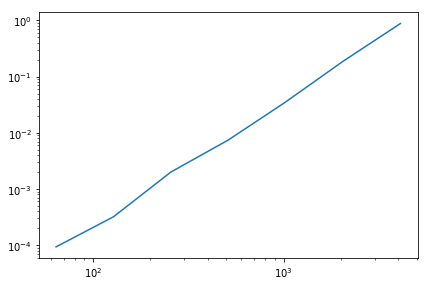
\includegraphics[width=0.75\textwidth]{1_1.png}
			\caption{Результат \texttt{analyze1()}}
			\label{fig:1.1}
		\end{figure}
		
		Наклон близок к 2, а не к 3, как ожидалось. Производительность np.linalg.solve почти квадратична в этом диапазоне размеров массива.
		
		
		Теперь поработаем с \texttt{analyze2()}
		\begin{lstlisting}[caption=Функция \texttt{analyze2()}]
			def analyze2(ys, fs, ts):
				args = np.outer(ts, fs)
				M = np.cos(PI2 * args)
				amps = np.dot(M, ys) / 2
				return amps
		\end{lstlisting}
		\begin{lstlisting}[caption=Работа с \texttt{analyze2()}]
			bests2 = run_speed_test(ns, analyze2)
			plot_bests(ns, bests2)
		\end{lstlisting}
		\begin{lstlisting}[caption=Результат, literate={µ}{$\upmu$}1 {±}{$\pm$}2]
			Output
			
			64
			54.4 µs ± 0 ns per loop (mean ± std. dev. of 1 run, 10000 loops each)
			128
			220 µs ± 0 ns per loop (mean ± std. dev. of 1 run, 10000 loops each)
			256
			1.18 ms ± 0 ns per loop (mean ± std. dev. of 1 run, 1000 loops each)
			512
			4.38 ms ± 0 ns per loop (mean ± std. dev. of 1 run, 100 loops each)
			1024
			16.7 ms ± 0 ns per loop (mean ± std. dev. of 1 run, 100 loops each)
			2048
			74.5 ms ± 0 ns per loop (mean ± std. dev. of 1 run, 10 loops each)
			4096
			307 ms ± 0 ns per loop (mean ± std. dev. of 1 run, 1 loop each)
			
			2.0723003647065377
		\end{lstlisting}
		
		\begin{figure}[H]
			\centering
			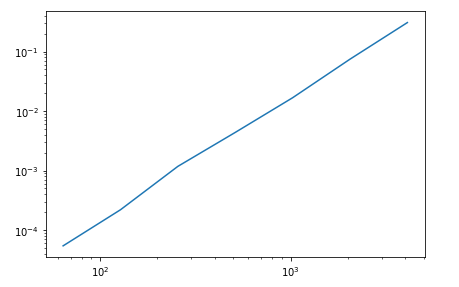
\includegraphics[width=0.75\textwidth]{1_2.png}
			\caption{Результат \texttt{analyze2()}}
			\label{fig:1.2}
		\end{figure}
		
		С analyze2() ситуация уже получше: наклон ближе к 2, как и ожидалось.
		
		Теперь поэкспериментируем c \texttt{scipy.fftpack.dct}
		
		\begin{lstlisting}[caption=Функция \texttt{scipy\_dct()}]
			import scipy.fftpack
			
			def scipy_dct(ys, freqs, ts):
				return scipy.fftpack.dct(ys, type=3)
		\end{lstlisting}
		\begin{lstlisting}[caption=Работа с \texttt{scipy\_dct()}]
			bests3 = run_speed_test(ns, scipy_dct)
			plot_bests(ns, bests3)
		\end{lstlisting}
		\begin{lstlisting}[caption=Результат, literate={µ}{$\upmu$}1 {±}{$\pm$}2]
			Output
			
			64
			7.48 µs ± 0 ns per loop (mean ± std. dev. of 1 run, 100000 loops each)
			128
			7.73 µs ± 0 ns per loop (mean ± std. dev. of 1 run, 100000 loops each)
			256
			8.44 µs ± 0 ns per loop (mean ± std. dev. of 1 run, 100000 loops each)
			512
			9.88 µs ± 0 ns per loop (mean ± std. dev. of 1 run, 100000 loops each)
			1024
			13 µs ± 0 ns per loop (mean ± std. dev. of 1 run, 100000 loops each)
			2048
			21.2 µs ± 0 ns per loop (mean ± std. dev. of 1 run, 10000 loops each)
			4096
			35.9 µs ± 0 ns per loop (mean ± std. dev. of 1 run, 10000 loops each)
			
		
			0.3686126799836147
		\end{lstlisting}
		
		\begin{figure}[H]
			\centering
			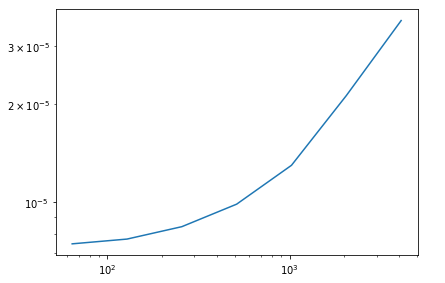
\includegraphics[width=0.75\textwidth]{1_3.png}
			\caption{Результат \texttt{scipy\_dct()}}
			\label{fig:1.3}
		\end{figure}
		
		Результат получили намного быстрее по времени, так как её асимптотическая сложность функции = \texttt{nlogn}
		
		Подведем итоги и отобразим все кривые на одном графике
		\begin{figure}[H]
			\centering
			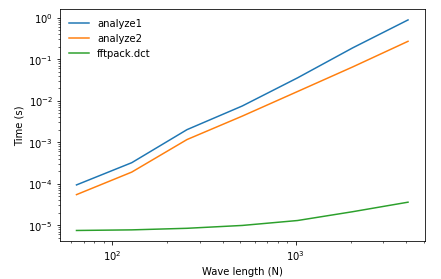
\includegraphics[width=0.75\textwidth]{1_4.png}
			\caption{Итог}
			\label{fig:1.4}
		\end{figure}
		
	\end{enumerate}
	\newpage
	
	
	\section {Упражение 6.2}
	
	\begin{enumerate} 
			
		\item \textbf{Задание}
			
		Реализуйте версию алгоритма ДКП - сжатие звука и изображений - и примените его для записи музыки и речи. Сколько компонент можно удалить до того, как разница станет заметной?
			
		\item \textbf{Ход работы}
			
		Возьмем звук саксофона из 5ой лабораторной работы и выделим из него сегмент
		\begin{lstlisting}[caption=Сегмент звука]
			from thinkdsp import read_wave
			
			wave = read_wave('100475__iluppai__saxophone-weep.wav')
			wave.make_audio()
			
			segment = wave.segment(start=1.2, duration=0.5)
			segment.normalize()
			segment.make_audio()
		\end{lstlisting}
	
		Теперь применим к сегменту ДКП
		\begin{lstlisting}[caption=Применяем ДКП]
			seg_dct = segment.make_dct()
			seg_dct.plot(high=4000)
			decorate(xlabel='Frequency (Hz)', ylabel='DCT')
		\end{lstlisting}
		\begin{figure}[H]
			\centering
			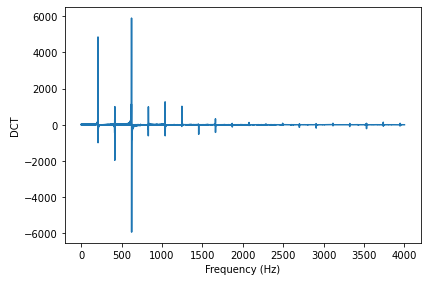
\includegraphics[width=0.75\textwidth]{2_1.png}
			\caption{Результат}
			\label{fig:2.1}
		\end{figure}
	
		По амплитуде выделяются мало гармоник, в основном большинство близки к нулю.
		
		Рассмотрим функцию \texttt{compress()}. Она принимает ДКП и значение порога и выставляет значение = 0 элементам, значение которых ниже порога (обрубает)
		
		\begin{lstlisting}[caption=Функция \texttt{compress()}]
			def compress(dct, thresh=1):
				count = 0
				for i, amp in enumerate(dct.amps):
					if np.abs(amp) < thresh:
						dct.hs[i] = 0
						count += 1
				
				n = len(dct.amps)
				print(count, n, 100 * count / n, sep='\t')
		\end{lstlisting}	
		
		Теперь попробуем сжать звук - применим функцию \texttt{compress()}
		\begin{lstlisting}[caption=Сжимаем звук]
			seg_dct = segment.make_dct()
			compress(seg_dct, thresh=10)
			seg_dct.plot(high=4000)
		\end{lstlisting}
		\begin{figure}[H]
			\centering
			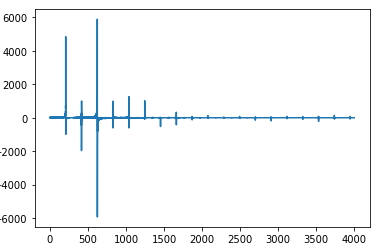
\includegraphics[width=0.75\textwidth]{2_2.png}
			\caption{Результат сжатия}
			\label{fig:2.2}
		\end{figure}
		
		Звук звучит точно также, как и до сжатия
		
		Чтобы применить ДКП для более длинного сегмента, рассмотрим функцию \texttt{make\_dct\_spectrogram()}. Она похожа на \texttt{wave.make\_spectorgram}, но в работе она использует ДКП.
		\begin{lstlisting}[caption=Функция \texttt{make\_dct\_spectrogram()}]
			from thinkdsp import Spectrogram
			
			def make_dct_spectrogram(wave, seg_length):
				window = np.hamming(seg_length)
				i, j = 0, seg_length
				step = seg_length // 2
				
				# map from time to Spectrum
				spec_map = {}
				
				while j < len(wave.ys):
					segment = wave.slice(i, j)
					segment.window(window)
					
					# the nominal time for this segment is the midpoint
					t = (segment.start + segment.end) / 2
					spec_map[t] = segment.make_dct()
					
					i += step
					j += step
				
				return Spectrogram(spec_map, seg_length)
		\end{lstlisting}
		
		Теперь применим её ко всему звуку
		\begin{lstlisting}[caption=Применяем \texttt{make\_dct\_spectrogram()}]
			spectro = make_dct_spectrogram(wave, seg_length=1024)
			for t, dct in sorted(spectro.spec_map.items()):
			compress(dct, thresh=0.2)
		\end{lstlisting}
		
		В большиснтве сегментов сжатие = 75\% - 80\%
		
		Теперь прослушаем результат
		\begin{lstlisting}[caption=Воспроизводим сжатый звук]
			wave2 = spectro.make_wave()
			wave2.make_audio()
		\end{lstlisting}
		
		В целом, звучание сохранилось, но появился сильно заметный разражающий треск на заднем фоне, который был еле слышен у несжатого звука.
		
	
	\end{enumerate}
	\newpage
		
		
	\section {Упражение 6.3}
		
	\begin{enumerate} 
				
		\item \textbf{Задание}
				
		Исследовать влияние фазы на восприятие звука. Поэкспериментировать с примерами.
				
		\item \textbf{Ход работы}
				
		В качестве звука для эксперимента возьмем звук саксофона из прошлого пункта и выделим из него сегмент.
		\begin{lstlisting}[caption=Сегмент звука саксофона]
			wave = read_wave('res/100475__iluppai__saxophone-weep.wav')
			wave.make_audio()
			segment = wave.segment(start=1.9, duration=0.6)
			
			spectrum = segment.make_spectrum()
			plot_three(spectrum, thresh=50)
		\end{lstlisting}
		
		Теперь отобразим
		1. Амплитуду сигнала
		2. Угловую часть спектра
		3. Форму волны
		
		\begin{figure}[H]
			\centering
			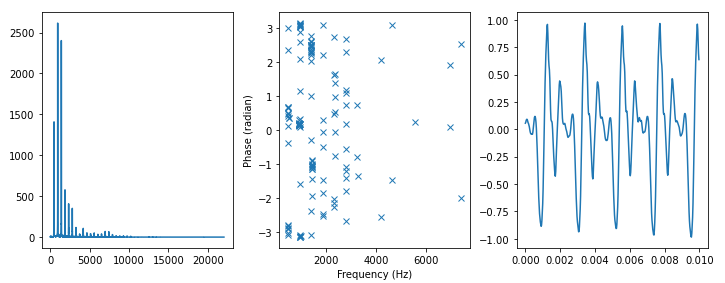
\includegraphics[width=0.75\textwidth]{3_1.png}
			\caption{Результат сжатия}
			\label{fig:3.1}
		\end{figure}	
		
		Теперь установим все углы на ноль
		\begin{lstlisting}[caption=Все углы на ноль]
			def zero_angle(spectrum):
				res = spectrum.copy()
				res.hs = res.amps
				return res
			
			spectrum2 = zero_angle(spectrum)
			plot_three(spectrum2, thresh=50)
		\end{lstlisting}
		\begin{figure}[H]
			\centering
			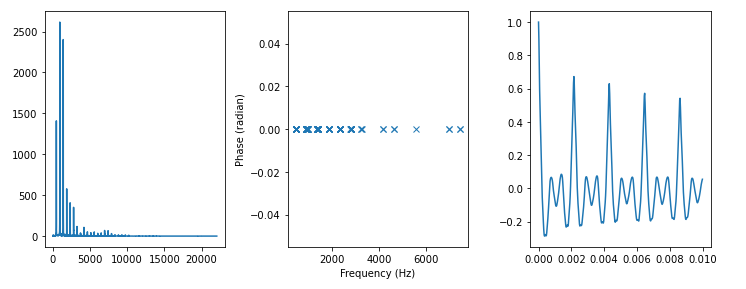
\includegraphics[width=0.75\textwidth]{3_2.png}
			\caption{Все углы на ноль}
			\label{fig:3.2}
		\end{figure}
		
		Амплитуда не изменилась, но изменилась форма волны. Теперь сегмент звучит волнообразно: сначала утихает, затем резко возрастает. Также звук стал тише.
		
		Теперь "повернем" углы на 1 радиан.
		\begin{lstlisting}[caption=Повернули углы]
			def rotate_angle(spectrum, offset):
				res = spectrum.copy()
				res.hs *= np.exp(1j * offset)
				return res
			
			spectrum3 = rotate_angle(spectrum, 1)
			plot_three(spectrum3, thresh=50)
		\end{lstlisting}
		\begin{figure}[H]
			\centering
			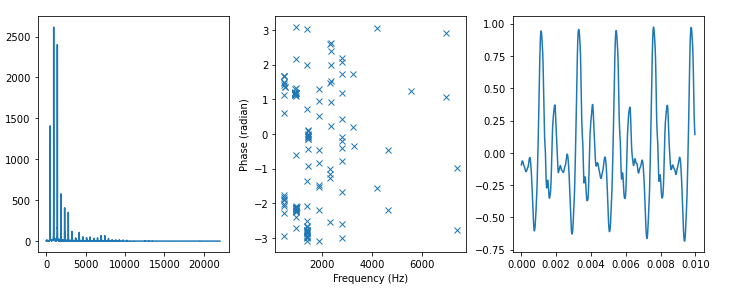
\includegraphics[width=0.75\textwidth]{3_3.png}
			\caption{Повернули углы}
			\label{fig:3.3}
		\end{figure}
		
		Звук нормализировался и звучит монотонно, по сравнению с прошлым результатом.
		
		Теперь пусть каддый угол будет равен случайному значению
		\begin{lstlisting}[caption=Рандомные углы]
			PI2 = np.pi * 2
			
			def random_angle(spectrum):
				res = spectrum.copy()
				angles = np.random.uniform(0, PI2, len(spectrum))
				res.hs *= np.exp(1j * angles)
				return res
			
			spectrum4 = random_angle(spectrum)
			plot_three(spectrum4, thresh=50)
		\end{lstlisting}
		\begin{figure}[H]
			\centering
			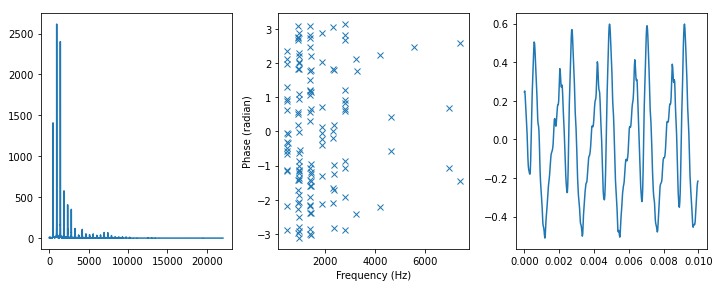
\includegraphics[width=0.75\textwidth]{3_4.png}
			\caption{Рандомные углы}
			\label{fig:3.4}
		\end{figure}
	
		Звук как-будто раздвоился, по сравнению с прошлым результатом.
		
		У звука саксофона есть особенность - основной компонент не является доминирующим. Фазовую структуру звуков в "пропавшей" частотой человеческое ухо может воспринимать. Автор предполагает, что ухо использует что-то вроде автокорреляции.
		
		
	\end{enumerate}
	\newpage
	
	
	\section {Вывод}
	
	В результате выполнения лабораторной работы получены навыки работы с дискретным косинусным преобразованием (ДКП). Также изучено влияние фазы на восприятие звука.
	

					
\end{document}